\documentclass[1p]{elsarticle_modified}
%\bibliographystyle{elsarticle-num}

%\usepackage[colorlinks]{hyperref}
%\usepackage{abbrmath_seonhwa} %\Abb, \Ascr, \Acal ,\Abf, \Afrak
\usepackage{amsfonts}
\usepackage{amssymb}
\usepackage{amsmath}
\usepackage{amsthm}
\usepackage{scalefnt}
\usepackage{amsbsy}
\usepackage{kotex}
\usepackage{caption}
\usepackage{subfig}
\usepackage{color}
\usepackage{graphicx}
\usepackage{xcolor} %% white, black, red, green, blue, cyan, magenta, yellow
\usepackage{float}
\usepackage{setspace}
\usepackage{hyperref}

\usepackage{tikz}
\usetikzlibrary{arrows}

\usepackage{multirow}
\usepackage{array} % fixed length table
\usepackage{hhline}

%%%%%%%%%%%%%%%%%%%%%
\makeatletter
\renewcommand*\env@matrix[1][\arraystretch]{%
	\edef\arraystretch{#1}%
	\hskip -\arraycolsep
	\let\@ifnextchar\new@ifnextchar
	\array{*\c@MaxMatrixCols c}}
\makeatother %https://tex.stackexchange.com/questions/14071/how-can-i-increase-the-line-spacing-in-a-matrix
%%%%%%%%%%%%%%%

\usepackage[normalem]{ulem}

\newcommand{\msout}[1]{\ifmmode\text{\sout{\ensuremath{#1}}}\else\sout{#1}\fi}
%SOURCE: \msout is \stkout macro in https://tex.stackexchange.com/questions/20609/strikeout-in-math-mode

\newcommand{\cancel}[1]{
	\ifmmode
	{\color{red}\msout{#1}}
	\else
	{\color{red}\sout{#1}}
	\fi
}

\newcommand{\add}[1]{
	{\color{blue}\uwave{#1}}
}

\newcommand{\replace}[2]{
	\ifmmode
	{\color{red}\msout{#1}}{\color{blue}\uwave{#2}}
	\else
	{\color{red}\sout{#1}}{\color{blue}\uwave{#2}}
	\fi
}

\newcommand{\Sol}{\mathcal{S}} %segment
\newcommand{\D}{D} %diagram
\newcommand{\A}{\mathcal{A}} %arc


%%%%%%%%%%%%%%%%%%%%%%%%%%%%%5 test

\def\sl{\operatorname{\textup{SL}}(2,\Cbb)}
\def\psl{\operatorname{\textup{PSL}}(2,\Cbb)}
\def\quan{\mkern 1mu \triangleright \mkern 1mu}

\theoremstyle{definition}
\newtheorem{thm}{Theorem}[section]
\newtheorem{prop}[thm]{Proposition}
\newtheorem{lem}[thm]{Lemma}
\newtheorem{ques}[thm]{Question}
\newtheorem{cor}[thm]{Corollary}
\newtheorem{defn}[thm]{Definition}
\newtheorem{exam}[thm]{Example}
\newtheorem{rmk}[thm]{Remark}
\newtheorem{alg}[thm]{Algorithm}

\newcommand{\I}{\sqrt{-1}}
\begin{document}

%\begin{frontmatter}
%
%\title{Boundary parabolic representations of knots up to 8 crossings}
%
%%% Group authors per affiliation:
%\author{Yunhi Cho} 
%\address{Department of Mathematics, University of Seoul, Seoul, Korea}
%\ead{yhcho@uos.ac.kr}
%
%
%\author{Seonhwa Kim} %\fnref{s_kim}}
%\address{Center for Geometry and Physics, Institute for Basic Science, Pohang, 37673, Korea}
%\ead{ryeona17@ibs.re.kr}
%
%\author{Hyuk Kim}
%\address{Department of Mathematical Sciences, Seoul National University, Seoul 08826, Korea}
%\ead{hyukkim@snu.ac.kr}
%
%\author{Seokbeom Yoon}
%\address{Department of Mathematical Sciences, Seoul National University, Seoul, 08826,  Korea}
%\ead{sbyoon15@snu.ac.kr}
%
%\begin{abstract}
%We find all boundary parabolic representation of knots up to 8 crossings.
%
%\end{abstract}
%\begin{keyword}
%    \MSC[2010] 57M25 
%\end{keyword}
%
%\end{frontmatter}

%\linenumbers
%\tableofcontents
%
\newcommand\colored[1]{\textcolor{white}{\rule[-0.35ex]{0.8em}{1.4ex}}\kern-0.8em\color{red} #1}%
%\newcommand\colored[1]{\textcolor{white}{ #1}\kern-2.17ex	\textcolor{white}{ #1}\kern-1.81ex	\textcolor{white}{ #1}\kern-2.15ex\color{red}#1	}

{\Large $\underline{12n_{0484}~(K12n_{0484})}$}

\setlength{\tabcolsep}{10pt}
\renewcommand{\arraystretch}{1.6}
\vspace{1cm}\begin{tabular}{m{100pt}>{\centering\arraybackslash}m{274pt}}
\multirow{5}{120pt}{
	\centering
	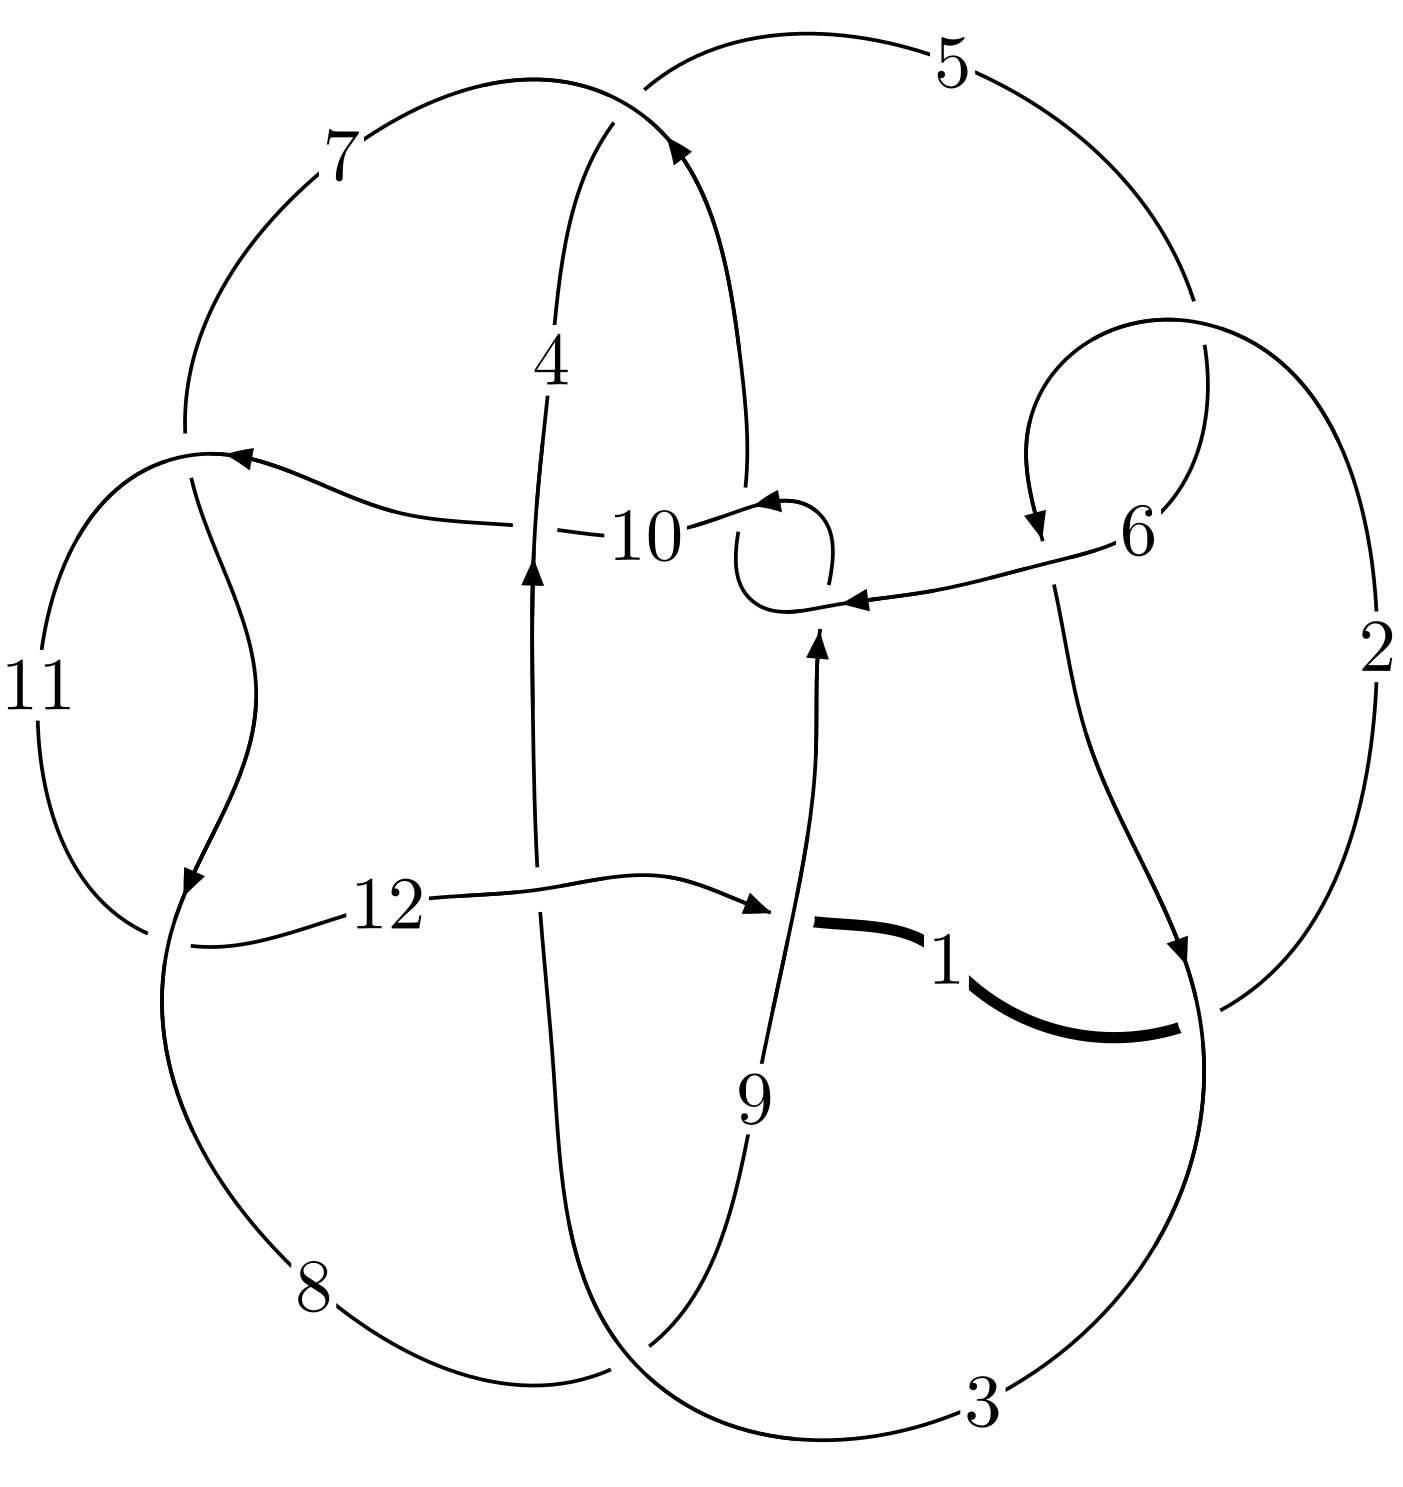
\includegraphics[width=112pt]{../../../GIT/diagram.site/Diagrams/png/2573_12n_0484.png}\\
\ \ \ A knot diagram\footnotemark}&
\allowdisplaybreaks
\textbf{Linearized knot diagam} \\
\cline{2-2}
 &
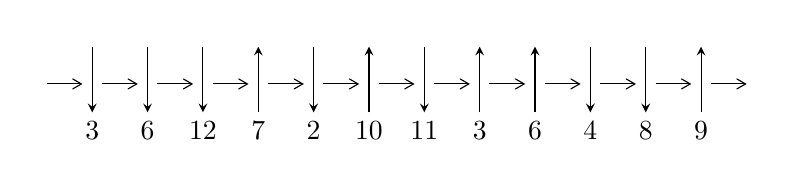
\begin{tikzpicture}[x=20pt, y=17pt]
	% nodes
	\node (C0) at (0, 0) {};
	\node (C1) at (1, 0) {};
	\node (C1U) at (1, +1) {};
	\node (C1D) at (1, -1) {3};

	\node (C2) at (2, 0) {};
	\node (C2U) at (2, +1) {};
	\node (C2D) at (2, -1) {6};

	\node (C3) at (3, 0) {};
	\node (C3U) at (3, +1) {};
	\node (C3D) at (3, -1) {12};

	\node (C4) at (4, 0) {};
	\node (C4U) at (4, +1) {};
	\node (C4D) at (4, -1) {7};

	\node (C5) at (5, 0) {};
	\node (C5U) at (5, +1) {};
	\node (C5D) at (5, -1) {2};

	\node (C6) at (6, 0) {};
	\node (C6U) at (6, +1) {};
	\node (C6D) at (6, -1) {10};

	\node (C7) at (7, 0) {};
	\node (C7U) at (7, +1) {};
	\node (C7D) at (7, -1) {11};

	\node (C8) at (8, 0) {};
	\node (C8U) at (8, +1) {};
	\node (C8D) at (8, -1) {3};

	\node (C9) at (9, 0) {};
	\node (C9U) at (9, +1) {};
	\node (C9D) at (9, -1) {6};

	\node (C10) at (10, 0) {};
	\node (C10U) at (10, +1) {};
	\node (C10D) at (10, -1) {4};

	\node (C11) at (11, 0) {};
	\node (C11U) at (11, +1) {};
	\node (C11D) at (11, -1) {8};

	\node (C12) at (12, 0) {};
	\node (C12U) at (12, +1) {};
	\node (C12D) at (12, -1) {9};
	\node (C13) at (13, 0) {};

	% arrows
	\draw[->,>={angle 60}]
	(C0) edge (C1) (C1) edge (C2) (C2) edge (C3) (C3) edge (C4) (C4) edge (C5) (C5) edge (C6) (C6) edge (C7) (C7) edge (C8) (C8) edge (C9) (C9) edge (C10) (C10) edge (C11) (C11) edge (C12) (C12) edge (C13) ;	\draw[->,>=stealth]
	(C1U) edge (C1D) (C2U) edge (C2D) (C3U) edge (C3D) (C4D) edge (C4U) (C5U) edge (C5D) (C6D) edge (C6U) (C7U) edge (C7D) (C8D) edge (C8U) (C9D) edge (C9U) (C10U) edge (C10D) (C11U) edge (C11D) (C12D) edge (C12U) ;
	\end{tikzpicture} \\
\hhline{~~} \\& 
\textbf{Solving Sequence} \\ \cline{2-2} 
 &
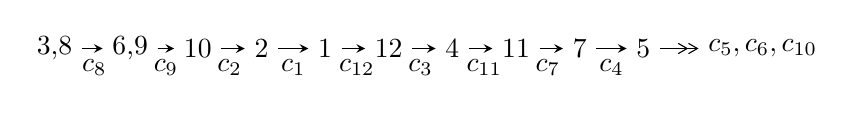
\begin{tikzpicture}[x=23pt, y=7pt]
	% node
	\node (A0) at (-1/8, 0) {3,8};
	\node (A1) at (17/16, 0) {6,9};
	\node (A2) at (17/8, 0) {10};
	\node (A3) at (25/8, 0) {2};
	\node (A4) at (33/8, 0) {1};
	\node (A5) at (41/8, 0) {12};
	\node (A6) at (49/8, 0) {4};
	\node (A7) at (57/8, 0) {11};
	\node (A8) at (65/8, 0) {7};
	\node (A9) at (73/8, 0) {5};
	\node (C1) at (1/2, -1) {$c_{8}$};
	\node (C2) at (13/8, -1) {$c_{9}$};
	\node (C3) at (21/8, -1) {$c_{2}$};
	\node (C4) at (29/8, -1) {$c_{1}$};
	\node (C5) at (37/8, -1) {$c_{12}$};
	\node (C6) at (45/8, -1) {$c_{3}$};
	\node (C7) at (53/8, -1) {$c_{11}$};
	\node (C8) at (61/8, -1) {$c_{7}$};
	\node (C9) at (69/8, -1) {$c_{4}$};
	\node (A10) at (11, 0) {$c_{5},c_{6},c_{10}$};

	% edge
	\draw[->,>=stealth]	
	(A0) edge (A1) (A1) edge (A2) (A2) edge (A3) (A3) edge (A4) (A4) edge (A5) (A5) edge (A6) (A6) edge (A7) (A7) edge (A8) (A8) edge (A9) ;
	\draw[->>,>={angle 60}]	
	(A9) edge (A10);
\end{tikzpicture} \\ 

\end{tabular} \\

\footnotetext{
The image of knot diagram is generated by the software ``\textbf{Draw programme}" developed by Andrew Bartholomew(\url{http://www.layer8.co.uk/maths/draw/index.htm\#Running-draw}), where we modified some parts for our purpose(\url{https://github.com/CATsTAILs/LinksPainter}).
}\phantom \\ \newline 
\centering \textbf{Ideals for irreducible components\footnotemark of $X_{\text{par}}$} 
 
\begin{align*}
I^u_{1}&=\langle 
-2.57724\times10^{98} u^{40}+8.25670\times10^{97} u^{39}+\cdots+1.32591\times10^{100} b+2.87003\times10^{100},\\
\phantom{I^u_{1}}&\phantom{= \langle  }-1.90566\times10^{100} u^{40}+7.67451\times10^{99} u^{39}+\cdots+1.84302\times10^{102} a-3.98069\times10^{102},\\
\phantom{I^u_{1}}&\phantom{= \langle  }2 u^{41}+59 u^{39}+\cdots-792 u-139\rangle \\
I^u_{2}&=\langle 
183 u^{10}+1583 u^9+\cdots+3889 b-2353,\;2799 u^{10}+10760 u^9+\cdots+3889 a+223,\\
\phantom{I^u_{2}}&\phantom{= \langle  }u^{11}+3 u^{10}+7 u^9+13 u^8+11 u^7+19 u^6+6 u^5+18 u^4+6 u^2-2 u+1\rangle \\
I^u_{3}&=\langle 
b+1,\;a-1,\;u+1\rangle \\
I^u_{4}&=\langle 
-2 u^3-2 u^2+2 b-3 u-3,\;-2 u^3+a-3 u-2,\;2 u^4+3 u^2+2 u+1\rangle \\
\\
\end{align*}
\raggedright * 4 irreducible components of $\dim_{\mathbb{C}}=0$, with total 57 representations.\\
\footnotetext{All coefficients of polynomials are rational numbers. But the coefficients are sometimes approximated in decimal forms when there is not enough margin.}
\newpage
\renewcommand{\arraystretch}{1}
\centering \section*{I. $I^u_{1}= \langle -2.58\times10^{98} u^{40}+8.26\times10^{97} u^{39}+\cdots+1.33\times10^{100} b+2.87\times10^{100},\;-1.91\times10^{100} u^{40}+7.67\times10^{99} u^{39}+\cdots+1.84\times10^{102} a-3.98\times10^{102},\;2 u^{41}+59 u^{39}+\cdots-792 u-139 \rangle$}
\flushleft \textbf{(i) Arc colorings}\\
\begin{tabular}{m{7pt} m{180pt} m{7pt} m{180pt} }
\flushright $a_{3}=$&$\begin{pmatrix}0\\u\end{pmatrix}$ \\
\flushright $a_{8}=$&$\begin{pmatrix}1\\0\end{pmatrix}$ \\
\flushright $a_{6}=$&$\begin{pmatrix}0.0103399 u^{40}-0.00416410 u^{39}+\cdots-1.23241 u+2.15988\\0.0194375 u^{40}-0.00622719 u^{39}+\cdots-11.2533 u-2.16457\end{pmatrix}$ \\
\flushright $a_{9}=$&$\begin{pmatrix}1\\- u^2\end{pmatrix}$ \\
\flushright $a_{10}=$&$\begin{pmatrix}-0.0209471 u^{40}+0.00485889 u^{39}+\cdots+19.6703 u+5.53621\\-0.00627194 u^{40}+0.00359880 u^{39}+\cdots+4.80640 u-0.268658\end{pmatrix}$ \\
\flushright $a_{2}=$&$\begin{pmatrix}-0.0223730 u^{40}+0.00212611 u^{39}+\cdots+18.5281 u+3.03016\\-0.00396870 u^{40}-0.00262692 u^{39}+\cdots+5.47182 u+1.30806\end{pmatrix}$ \\
\flushright $a_{1}=$&$\begin{pmatrix}-0.0223730 u^{40}+0.00212611 u^{39}+\cdots+18.5281 u+3.03016\\-0.00307852 u^{40}-0.00354962 u^{39}+\cdots+6.18480 u+1.16029\end{pmatrix}$ \\
\flushright $a_{12}=$&$\begin{pmatrix}-0.0184043 u^{40}+0.00475303 u^{39}+\cdots+13.0562 u+1.72210\\-0.000584007 u^{40}-0.00418261 u^{39}+\cdots+4.86872 u+0.977723\end{pmatrix}$ \\
\flushright $a_{4}=$&$\begin{pmatrix}-0.0191133 u^{40}+0.00882757 u^{39}+\cdots+0.506034 u-0.758338\\0.00679681 u^{40}-0.00471144 u^{39}+\cdots-3.46799 u-0.799858\end{pmatrix}$ \\
\flushright $a_{11}=$&$\begin{pmatrix}-0.0189883 u^{40}+0.000570424 u^{39}+\cdots+17.9250 u+2.69983\\-0.000584007 u^{40}-0.00418261 u^{39}+\cdots+4.86872 u+0.977723\end{pmatrix}$ \\
\flushright $a_{7}=$&$\begin{pmatrix}-0.000436229 u^{40}-0.00330818 u^{39}+\cdots+6.39844 u+2.38333\\0.0110725 u^{40}-0.0101050 u^{39}+\cdots-0.426320 u+1.29385\end{pmatrix}$ \\
\flushright $a_{5}=$&$\begin{pmatrix}-0.00336300 u^{40}+0.00725991 u^{39}+\cdots-12.4525 u-5.75232\\-0.0229539 u^{40}+0.00793740 u^{39}+\cdots+12.3051 u+2.17246\end{pmatrix}$\\&\end{tabular}
\flushleft \textbf{(ii) Obstruction class $= -1$}\\~\\
\flushleft \textbf{(iii) Cusp Shapes $= 0.0503579 u^{40}-0.0337763 u^{39}+\cdots-41.9472 u-6.50005$}\\~\\
\newpage\renewcommand{\arraystretch}{1}
\flushleft \textbf{(iv) u-Polynomials at the component}\newline \\
\begin{tabular}{m{50pt}|m{274pt}}
Crossings & \hspace{64pt}u-Polynomials at each crossing \\
\hline $$\begin{aligned}c_{1}\end{aligned}$$&$\begin{aligned}
&u^{41}+62 u^{40}+\cdots+20980954 u+3066001
\end{aligned}$\\
\hline $$\begin{aligned}c_{2},c_{5}\end{aligned}$$&$\begin{aligned}
&u^{41}-2 u^{40}+\cdots-994 u+1751
\end{aligned}$\\
\hline $$\begin{aligned}c_{3}\end{aligned}$$&$\begin{aligned}
&u^{41}-7 u^{40}+\cdots-32 u+2
\end{aligned}$\\
\hline $$\begin{aligned}c_{4}\end{aligned}$$&$\begin{aligned}
&u^{41}+8 u^{40}+\cdots+202 u+482
\end{aligned}$\\
\hline $$\begin{aligned}c_{6},c_{9}\end{aligned}$$&$\begin{aligned}
&u^{41}-4 u^{40}+\cdots-532 u-484
\end{aligned}$\\
\hline $$\begin{aligned}c_{7},c_{11}\end{aligned}$$&$\begin{aligned}
&u^{41}-18 u^{39}+\cdots-147 u-9
\end{aligned}$\\
\hline $$\begin{aligned}c_{8}\end{aligned}$$&$\begin{aligned}
&2(2 u^{41}+59 u^{39}+\cdots-792 u+139)
\end{aligned}$\\
\hline $$\begin{aligned}c_{10}\end{aligned}$$&$\begin{aligned}
&2(2 u^{41}+4 u^{40}+\cdots+12 u-1)
\end{aligned}$\\
\hline $$\begin{aligned}c_{12}\end{aligned}$$&$\begin{aligned}
&u^{41}+50 u^{39}+\cdots+3836088 u+323212
\end{aligned}$\\
\hline
\end{tabular}\\~\\
\newpage\renewcommand{\arraystretch}{1}
\flushleft \textbf{(v) Riley Polynomials at the component}\newline \\
\begin{tabular}{m{50pt}|m{274pt}}
Crossings & \hspace{64pt}Riley Polynomials at each crossing \\
\hline $$\begin{aligned}c_{1}\end{aligned}$$&$\begin{aligned}
&y^{41}-174 y^{40}+\cdots-176579932485582 y-9400362132001
\end{aligned}$\\
\hline $$\begin{aligned}c_{2},c_{5}\end{aligned}$$&$\begin{aligned}
&y^{41}-62 y^{40}+\cdots+20980954 y-3066001
\end{aligned}$\\
\hline $$\begin{aligned}c_{3}\end{aligned}$$&$\begin{aligned}
&y^{41}-7 y^{40}+\cdots+68 y-4
\end{aligned}$\\
\hline $$\begin{aligned}c_{4}\end{aligned}$$&$\begin{aligned}
&y^{41}+26 y^{40}+\cdots-2659360 y-232324
\end{aligned}$\\
\hline $$\begin{aligned}c_{6},c_{9}\end{aligned}$$&$\begin{aligned}
&y^{41}+50 y^{39}+\cdots-1201888 y-234256
\end{aligned}$\\
\hline $$\begin{aligned}c_{7},c_{11}\end{aligned}$$&$\begin{aligned}
&y^{41}-36 y^{40}+\cdots+6831 y-81
\end{aligned}$\\
\hline $$\begin{aligned}c_{8}\end{aligned}$$&$\begin{aligned}
&4(4 y^{41}+236 y^{40}+\cdots-158364 y-19321)
\end{aligned}$\\
\hline $$\begin{aligned}c_{10}\end{aligned}$$&$\begin{aligned}
&4(4 y^{41}+36 y^{40}+\cdots+32 y-1)
\end{aligned}$\\
\hline $$\begin{aligned}c_{12}\end{aligned}$$&$\begin{aligned}
&y^{41}+100 y^{40}+\cdots+6045979389712 y-104465996944
\end{aligned}$\\
\hline
\end{tabular}\\~\\
\newpage\flushleft \textbf{(vi) Complex Volumes and Cusp Shapes}
$$\begin{array}{c|c|c}  
\text{Solutions to }I^u_{1}& \I (\text{vol} + \sqrt{-1}CS) & \text{Cusp shape}\\
 \hline 
\begin{aligned}
u &= -0.659232 + 0.776800 I \\
a &= \phantom{-}0.577914 + 0.165637 I \\
b &= -0.024468 - 0.254653 I\end{aligned}
 & -0.03579 - 2.12702 I & -2.30724 + 6.34493 I \\ \hline\begin{aligned}
u &= -0.659232 - 0.776800 I \\
a &= \phantom{-}0.577914 - 0.165637 I \\
b &= -0.024468 + 0.254653 I\end{aligned}
 & -0.03579 + 2.12702 I & -2.30724 - 6.34493 I \\ \hline\begin{aligned}
u &= \phantom{-}0.393962 + 0.883594 I \\
a &= \phantom{-}0.541007 - 0.684990 I \\
b &= \phantom{-}1.124350 - 0.835430 I\end{aligned}
 & \phantom{-}3.52455 - 0.44279 I & \phantom{-}1.64463 + 0.69069 I \\ \hline\begin{aligned}
u &= \phantom{-}0.393962 - 0.883594 I \\
a &= \phantom{-}0.541007 + 0.684990 I \\
b &= \phantom{-}1.124350 + 0.835430 I\end{aligned}
 & \phantom{-}3.52455 + 0.44279 I & \phantom{-}1.64463 - 0.69069 I \\ \hline\begin{aligned}
u &= \phantom{-}0.254000 + 1.050130 I \\
a &= -1.31930 + 0.64361 I \\
b &= -0.809991 + 0.134439 I\end{aligned}
 & -5.50368 - 6.18013 I & -6.07543 + 4.97240 I \\ \hline\begin{aligned}
u &= \phantom{-}0.254000 - 1.050130 I \\
a &= -1.31930 - 0.64361 I \\
b &= -0.809991 - 0.134439 I\end{aligned}
 & -5.50368 + 6.18013 I & -6.07543 - 4.97240 I \\ \hline\begin{aligned}
u &= -0.343509 + 0.778339 I \\
a &= -1.50036 - 0.93858 I \\
b &= -0.597196 - 0.150858 I\end{aligned}
 & -5.88104 - 0.44141 I & -6.92109 + 1.29385 I \\ \hline\begin{aligned}
u &= -0.343509 - 0.778339 I \\
a &= -1.50036 + 0.93858 I \\
b &= -0.597196 + 0.150858 I\end{aligned}
 & -5.88104 + 0.44141 I & -6.92109 - 1.29385 I \\ \hline\begin{aligned}
u &= \phantom{-}0.432526 + 0.728373 I \\
a &= \phantom{-}0.847277 - 0.498164 I \\
b &= -0.263708 - 0.214377 I\end{aligned}
 & -1.32932 - 0.71050 I & -7.34406 + 3.00260 I \\ \hline\begin{aligned}
u &= \phantom{-}0.432526 - 0.728373 I \\
a &= \phantom{-}0.847277 + 0.498164 I \\
b &= -0.263708 + 0.214377 I\end{aligned}
 & -1.32932 + 0.71050 I & -7.34406 - 3.00260 I\\
 \hline 
 \end{array}$$\newpage$$\begin{array}{c|c|c}  
\text{Solutions to }I^u_{1}& \I (\text{vol} + \sqrt{-1}CS) & \text{Cusp shape}\\
 \hline 
\begin{aligned}
u &= \phantom{-}0.786645\phantom{ +0.000000I} \\
a &= \phantom{-}1.52147\phantom{ +0.000000I} \\
b &= -0.499922\phantom{ +0.000000I}\end{aligned}
 & -2.75131\phantom{ +0.000000I} & \phantom{-}5.92420\phantom{ +0.000000I} \\ \hline\begin{aligned}
u &= \phantom{-}0.572393 + 0.467249 I \\
a &= \phantom{-}0.784322 + 0.182815 I \\
b &= -0.577015 - 1.030610 I\end{aligned}
 & -2.75470 - 0.87273 I & -3.72912 + 1.33601 I \\ \hline\begin{aligned}
u &= \phantom{-}0.572393 - 0.467249 I \\
a &= \phantom{-}0.784322 - 0.182815 I \\
b &= -0.577015 + 1.030610 I\end{aligned}
 & -2.75470 + 0.87273 I & -3.72912 - 1.33601 I \\ \hline\begin{aligned}
u &= -0.416524 + 1.237420 I \\
a &= \phantom{-}0.408598 - 0.403112 I \\
b &= -0.286242 - 0.497821 I\end{aligned}
 & -0.89253 - 2.94273 I & \phantom{-0.000000 } 0 \\ \hline\begin{aligned}
u &= -0.416524 - 1.237420 I \\
a &= \phantom{-}0.408598 + 0.403112 I \\
b &= -0.286242 + 0.497821 I\end{aligned}
 & -0.89253 + 2.94273 I & \phantom{-0.000000 } 0 \\ \hline\begin{aligned}
u &= -0.534052 + 0.272508 I \\
a &= \phantom{-}1.35667 + 0.56380 I \\
b &= \phantom{-}0.977815 - 0.039583 I\end{aligned}
 & \phantom{-}2.14913 - 0.81916 I & \phantom{-}6.43098 + 7.00832 I \\ \hline\begin{aligned}
u &= -0.534052 - 0.272508 I \\
a &= \phantom{-}1.35667 - 0.56380 I \\
b &= \phantom{-}0.977815 + 0.039583 I\end{aligned}
 & \phantom{-}2.14913 + 0.81916 I & \phantom{-}6.43098 - 7.00832 I \\ \hline\begin{aligned}
u &= \phantom{-}0.171734 + 0.527077 I \\
a &= \phantom{-}0.88599 + 1.93343 I \\
b &= -0.381893 + 0.315896 I\end{aligned}
 & \phantom{-}4.54292 + 2.96089 I & -5.84505 - 9.32253 I \\ \hline\begin{aligned}
u &= \phantom{-}0.171734 - 0.527077 I \\
a &= \phantom{-}0.88599 - 1.93343 I \\
b &= -0.381893 - 0.315896 I\end{aligned}
 & \phantom{-}4.54292 - 2.96089 I & -5.84505 + 9.32253 I \\ \hline\begin{aligned}
u &= \phantom{-}1.04509 + 1.16303 I \\
a &= -0.575660 + 0.408131 I \\
b &= \phantom{-}0.336966 + 0.467880 I\end{aligned}
 & -4.77375 + 7.71761 I & \phantom{-0.000000 } 0\\
 \hline 
 \end{array}$$\newpage$$\begin{array}{c|c|c}  
\text{Solutions to }I^u_{1}& \I (\text{vol} + \sqrt{-1}CS) & \text{Cusp shape}\\
 \hline 
\begin{aligned}
u &= \phantom{-}1.04509 - 1.16303 I \\
a &= -0.575660 - 0.408131 I \\
b &= \phantom{-}0.336966 - 0.467880 I\end{aligned}
 & -4.77375 - 7.71761 I & \phantom{-0.000000 } 0 \\ \hline\begin{aligned}
u &= -0.356665 + 0.207131 I \\
a &= \phantom{-}1.12852 - 1.40117 I \\
b &= -0.933888 + 0.923317 I\end{aligned}
 & -1.64023 - 6.11163 I & -0.87211 + 3.36095 I \\ \hline\begin{aligned}
u &= -0.356665 - 0.207131 I \\
a &= \phantom{-}1.12852 + 1.40117 I \\
b &= -0.933888 - 0.923317 I\end{aligned}
 & -1.64023 + 6.11163 I & -0.87211 - 3.36095 I \\ \hline\begin{aligned}
u &= -0.241179 + 0.293581 I \\
a &= \phantom{-}1.84296 - 0.32729 I \\
b &= \phantom{-}0.998293 - 0.269510 I\end{aligned}
 & \phantom{-}1.88617 - 0.91020 I & \phantom{-}6.79810 - 1.89134 I \\ \hline\begin{aligned}
u &= -0.241179 - 0.293581 I \\
a &= \phantom{-}1.84296 + 0.32729 I \\
b &= \phantom{-}0.998293 + 0.269510 I\end{aligned}
 & \phantom{-}1.88617 + 0.91020 I & \phantom{-}6.79810 + 1.89134 I \\ \hline\begin{aligned}
u &= \phantom{-}0.18824 + 1.62909 I \\
a &= -0.155518 + 1.166050 I \\
b &= \phantom{-}0.00435 + 2.45451 I\end{aligned}
 & -8.69666 + 3.51054 I & \phantom{-0.000000 } 0 \\ \hline\begin{aligned}
u &= \phantom{-}0.18824 - 1.62909 I \\
a &= -0.155518 - 1.166050 I \\
b &= \phantom{-}0.00435 - 2.45451 I\end{aligned}
 & -8.69666 - 3.51054 I & \phantom{-0.000000 } 0 \\ \hline\begin{aligned}
u &= -0.30115 + 1.75023 I \\
a &= \phantom{-}0.062139 + 1.105720 I \\
b &= \phantom{-}0.52944 + 2.26135 I\end{aligned}
 & -14.5520 - 3.8090 I & \phantom{-0.000000 } 0 \\ \hline\begin{aligned}
u &= -0.30115 - 1.75023 I \\
a &= \phantom{-}0.062139 - 1.105720 I \\
b &= \phantom{-}0.52944 - 2.26135 I\end{aligned}
 & -14.5520 + 3.8090 I & \phantom{-0.000000 } 0 \\ \hline\begin{aligned}
u &= -0.24365 + 1.79461 I \\
a &= \phantom{-}0.005218 - 1.222810 I \\
b &= \phantom{-}0.03876 - 2.26816 I\end{aligned}
 & -9.19332 - 6.12722 I & \phantom{-0.000000 } 0\\
 \hline 
 \end{array}$$\newpage$$\begin{array}{c|c|c}  
\text{Solutions to }I^u_{1}& \I (\text{vol} + \sqrt{-1}CS) & \text{Cusp shape}\\
 \hline 
\begin{aligned}
u &= -0.24365 - 1.79461 I \\
a &= \phantom{-}0.005218 + 1.222810 I \\
b &= \phantom{-}0.03876 + 2.26816 I\end{aligned}
 & -9.19332 + 6.12722 I & \phantom{-0.000000 } 0 \\ \hline\begin{aligned}
u &= \phantom{-}0.16879 + 1.88364 I \\
a &= -0.044736 - 1.118060 I \\
b &= \phantom{-}0.35074 - 2.24460 I\end{aligned}
 & -16.2241 - 3.4621 I & \phantom{-0.000000 } 0 \\ \hline\begin{aligned}
u &= \phantom{-}0.16879 - 1.88364 I \\
a &= -0.044736 + 1.118060 I \\
b &= \phantom{-}0.35074 + 2.24460 I\end{aligned}
 & -16.2241 + 3.4621 I & \phantom{-0.000000 } 0 \\ \hline\begin{aligned}
u &= \phantom{-}0.32422 + 1.88669 I \\
a &= -0.053583 + 0.940689 I \\
b &= -0.11454 + 2.30108 I\end{aligned}
 & -10.43640 + 3.80935 I & \phantom{-0.000000 } 0 \\ \hline\begin{aligned}
u &= \phantom{-}0.32422 - 1.88669 I \\
a &= -0.053583 - 0.940689 I \\
b &= -0.11454 - 2.30108 I\end{aligned}
 & -10.43640 - 3.80935 I & \phantom{-0.000000 } 0 \\ \hline\begin{aligned}
u &= \phantom{-}0.32406 + 1.92161 I \\
a &= -0.072428 - 1.055780 I \\
b &= -0.14431 - 2.43176 I\end{aligned}
 & -15.2118 + 13.8525 I & \phantom{-0.000000 } 0 \\ \hline\begin{aligned}
u &= \phantom{-}0.32406 - 1.92161 I \\
a &= -0.072428 + 1.055780 I \\
b &= -0.14431 + 2.43176 I\end{aligned}
 & -15.2118 - 13.8525 I & \phantom{-0.000000 } 0 \\ \hline\begin{aligned}
u &= -0.17851 + 2.01135 I \\
a &= -0.115497 + 0.968666 I \\
b &= -0.18704 + 2.37176 I\end{aligned}
 & -16.2944 - 5.5634 I & \phantom{-0.000000 } 0 \\ \hline\begin{aligned}
u &= -0.17851 - 2.01135 I \\
a &= -0.115497 - 0.968666 I \\
b &= -0.18704 - 2.37176 I\end{aligned}
 & -16.2944 + 5.5634 I & \phantom{-0.000000 } 0 \\ \hline\begin{aligned}
u &= -0.99386 + 1.82091 I \\
a &= -0.349882 - 0.371487 I \\
b &= \phantom{-}0.70955 - 1.54548 I\end{aligned}
 & -3.40570 + 0.32734 I & \phantom{-0.000000 } 0\\
 \hline 
 \end{array}$$\newpage$$\begin{array}{c|c|c}  
\text{Solutions to }I^u_{1}& \I (\text{vol} + \sqrt{-1}CS) & \text{Cusp shape}\\
 \hline 
\begin{aligned}
u &= -0.99386 - 1.82091 I \\
a &= -0.349882 + 0.371487 I \\
b &= \phantom{-}0.70955 + 1.54548 I\end{aligned}
 & -3.40570 - 0.32734 I & \phantom{-0.000000 } 0\\
 \hline 
 \end{array}$$\newpage\newpage\renewcommand{\arraystretch}{1}
\centering \section*{II. $I^u_{2}= \langle 183 u^{10}+1583 u^9+\cdots+3889 b-2353,\;2799 u^{10}+10760 u^9+\cdots+3889 a+223,\;u^{11}+3 u^{10}+\cdots-2 u+1 \rangle$}
\flushleft \textbf{(i) Arc colorings}\\
\begin{tabular}{m{7pt} m{180pt} m{7pt} m{180pt} }
\flushright $a_{3}=$&$\begin{pmatrix}0\\u\end{pmatrix}$ \\
\flushright $a_{8}=$&$\begin{pmatrix}1\\0\end{pmatrix}$ \\
\flushright $a_{6}=$&$\begin{pmatrix}-0.719722 u^{10}-2.76678 u^{9}+\cdots-5.35485 u-0.0573412\\-0.0470558 u^{10}-0.407046 u^{9}+\cdots-0.206480 u+0.605040\end{pmatrix}$ \\
\flushright $a_{9}=$&$\begin{pmatrix}1\\- u^2\end{pmatrix}$ \\
\flushright $a_{10}=$&$\begin{pmatrix}0.582926 u^{10}+2.36488 u^{9}+\cdots+6.37208 u+1.15505\\-0.136796 u^{10}-0.401903 u^{9}+\cdots+1.01723 u-0.902289\end{pmatrix}$ \\
\flushright $a_{2}=$&$\begin{pmatrix}-0.622011 u^{10}-2.33685 u^{9}+\cdots-4.65287 u-2.26999\\-0.556956 u^{10}-1.85060 u^{9}+\cdots-0.00128568 u+0.112111\end{pmatrix}$ \\
\flushright $a_{1}=$&$\begin{pmatrix}-0.622011 u^{10}-2.33685 u^{9}+\cdots-4.65287 u-2.26999\\-0.497814 u^{10}-1.59038 u^{9}+\cdots+0.318334 u-0.358704\end{pmatrix}$ \\
\flushright $a_{12}=$&$\begin{pmatrix}-0.0650553 u^{10}-0.486243 u^{9}+\cdots-4.65158 u-2.38210\\-0.349447 u^{10}-1.13757 u^{9}+\cdots+0.515814 u-0.178966\end{pmatrix}$ \\
\flushright $a_{4}=$&$\begin{pmatrix}-2.03626 u^{10}-6.55953 u^{9}+\cdots-8.33942 u+3.59733\\0.212651 u^{10}+0.735665 u^{9}+\cdots+1.50141 u+0.276678\end{pmatrix}$ \\
\flushright $a_{11}=$&$\begin{pmatrix}-0.414502 u^{10}-1.62381 u^{9}+\cdots-4.13577 u-2.56107\\-0.349447 u^{10}-1.13757 u^{9}+\cdots+0.515814 u-0.178966\end{pmatrix}$ \\
\flushright $a_{7}=$&$\begin{pmatrix}-0.0105426 u^{10}-0.446387 u^{9}+\cdots+1.58215 u+1.43610\\0.266135 u^{10}+0.170995 u^{9}+\cdots+1.93829 u-0.618668\end{pmatrix}$ \\
\flushright $a_{5}=$&$\begin{pmatrix}-1.32142 u^{10}-4.41425 u^{9}+\cdots-3.51967 u+3.51530\\0.286192 u^{10}+0.459244 u^{9}+\cdots+2.97711 u-0.204423\end{pmatrix}$\\&\end{tabular}
\flushleft \textbf{(ii) Obstruction class $= 1$}\\~\\
\flushleft \textbf{(iii) Cusp Shapes $= -\frac{9564}{3889} u^{10}-\frac{28859}{3889} u^9-\frac{63016}{3889} u^8-\frac{109107}{3889} u^7-\frac{66615}{3889} u^6-\frac{107750}{3889} u^5+\frac{13439}{3889} u^4-\frac{81002}{3889} u^3+\frac{23490}{3889} u^2+\frac{22170}{3889} u+\frac{11276}{3889}$}\\~\\
\newpage\renewcommand{\arraystretch}{1}
\flushleft \textbf{(iv) u-Polynomials at the component}\newline \\
\begin{tabular}{m{50pt}|m{274pt}}
Crossings & \hspace{64pt}u-Polynomials at each crossing \\
\hline $$\begin{aligned}c_{1}\end{aligned}$$&$\begin{aligned}
&u^{11}-8 u^{10}+\cdots-16 u^2-1
\end{aligned}$\\
\hline $$\begin{aligned}c_{2}\end{aligned}$$&$\begin{aligned}
&u^{11}+6 u^{10}+14 u^9+16 u^8+8 u^7- u^6-3 u^5-4 u^4-7 u^3-8 u^2-4 u-1
\end{aligned}$\\
\hline $$\begin{aligned}c_{3}\end{aligned}$$&$\begin{aligned}
&u^{11}+3 u^{10}+\cdots+5 u+1
\end{aligned}$\\
\hline $$\begin{aligned}c_{4}\end{aligned}$$&$\begin{aligned}
&u^{11}+2 u^{10}+\cdots+2 u-1
\end{aligned}$\\
\hline $$\begin{aligned}c_{5}\end{aligned}$$&$\begin{aligned}
&u^{11}-6 u^{10}+14 u^9-16 u^8+8 u^7+u^6-3 u^5+4 u^4-7 u^3+8 u^2-4 u+1
\end{aligned}$\\
\hline $$\begin{aligned}c_{6}\end{aligned}$$&$\begin{aligned}
&u^{11}-3 u^{10}+u^9+7 u^8-8 u^7-5 u^6+12 u^5+2 u^4-10 u^3+5 u-1
\end{aligned}$\\
\hline $$\begin{aligned}c_{7}\end{aligned}$$&$\begin{aligned}
&u^{11}-3 u^9-4 u^8+2 u^7+11 u^6+12 u^5-5 u^4-11 u^3-10 u^2+7 u-1
\end{aligned}$\\
\hline $$\begin{aligned}c_{8}\end{aligned}$$&$\begin{aligned}
&u^{11}+3 u^{10}+7 u^9+13 u^8+11 u^7+19 u^6+6 u^5+18 u^4+6 u^2-2 u+1
\end{aligned}$\\
\hline $$\begin{aligned}c_{9}\end{aligned}$$&$\begin{aligned}
&u^{11}+3 u^{10}+u^9-7 u^8-8 u^7+5 u^6+12 u^5-2 u^4-10 u^3+5 u+1
\end{aligned}$\\
\hline $$\begin{aligned}c_{10}\end{aligned}$$&$\begin{aligned}
&u^{11}+3 u^{10}+4 u^9+7 u^8+6 u^7+8 u^6+u^5+6 u^4+2 u^3+2 u^2+1
\end{aligned}$\\
\hline $$\begin{aligned}c_{11}\end{aligned}$$&$\begin{aligned}
&u^{11}-3 u^9+4 u^8+2 u^7-11 u^6+12 u^5+5 u^4-11 u^3+10 u^2+7 u+1
\end{aligned}$\\
\hline $$\begin{aligned}c_{12}\end{aligned}$$&$\begin{aligned}
&u^{11}- u^{10}+11 u^9+26 u^7+29 u^6+35 u^5+42 u^4+37 u^3+14 u^2+4 u-1
\end{aligned}$\\
\hline
\end{tabular}\\~\\
\newpage\renewcommand{\arraystretch}{1}
\flushleft \textbf{(v) Riley Polynomials at the component}\newline \\
\begin{tabular}{m{50pt}|m{274pt}}
Crossings & \hspace{64pt}Riley Polynomials at each crossing \\
\hline $$\begin{aligned}c_{1}\end{aligned}$$&$\begin{aligned}
&y^{11}-24 y^{10}+\cdots-32 y-1
\end{aligned}$\\
\hline $$\begin{aligned}c_{2},c_{5}\end{aligned}$$&$\begin{aligned}
&y^{11}-8 y^{10}+\cdots-16 y^2-1
\end{aligned}$\\
\hline $$\begin{aligned}c_{3}\end{aligned}$$&$\begin{aligned}
&y^{11}+y^{10}+\cdots+7 y-1
\end{aligned}$\\
\hline $$\begin{aligned}c_{4}\end{aligned}$$&$\begin{aligned}
&y^{11}+2 y^{10}+\cdots-2 y-1
\end{aligned}$\\
\hline $$\begin{aligned}c_{6},c_{9}\end{aligned}$$&$\begin{aligned}
&y^{11}-7 y^{10}+\cdots+25 y-1
\end{aligned}$\\
\hline $$\begin{aligned}c_{7},c_{11}\end{aligned}$$&$\begin{aligned}
&y^{11}-6 y^{10}+\cdots+29 y-1
\end{aligned}$\\
\hline $$\begin{aligned}c_{8}\end{aligned}$$&$\begin{aligned}
&y^{11}+5 y^{10}+\cdots-8 y-1
\end{aligned}$\\
\hline $$\begin{aligned}c_{10}\end{aligned}$$&$\begin{aligned}
&y^{11}- y^{10}+\cdots-4 y-1
\end{aligned}$\\
\hline $$\begin{aligned}c_{12}\end{aligned}$$&$\begin{aligned}
&y^{11}+21 y^{10}+\cdots+44 y-1
\end{aligned}$\\
\hline
\end{tabular}\\~\\
\newpage\flushleft \textbf{(vi) Complex Volumes and Cusp Shapes}
$$\begin{array}{c|c|c}  
\text{Solutions to }I^u_{2}& \I (\text{vol} + \sqrt{-1}CS) & \text{Cusp shape}\\
 \hline 
\begin{aligned}
u &= \phantom{-}0.480135 + 0.881380 I \\
a &= -0.153776 - 0.485356 I \\
b &= -1.41525 - 0.50524 I\end{aligned}
 & -2.33883 + 7.37149 I & -3.11706 - 6.99331 I \\ \hline\begin{aligned}
u &= \phantom{-}0.480135 - 0.881380 I \\
a &= -0.153776 + 0.485356 I \\
b &= -1.41525 + 0.50524 I\end{aligned}
 & -2.33883 - 7.37149 I & -3.11706 + 6.99331 I \\ \hline\begin{aligned}
u &= -0.264154 + 0.702912 I \\
a &= \phantom{-}1.116630 + 0.190741 I \\
b &= \phantom{-}1.138780 - 0.052004 I\end{aligned}
 & \phantom{-}1.51158 - 1.27486 I & -4.85663 + 8.07328 I \\ \hline\begin{aligned}
u &= -0.264154 - 0.702912 I \\
a &= \phantom{-}1.116630 - 0.190741 I \\
b &= \phantom{-}1.138780 + 0.052004 I\end{aligned}
 & \phantom{-}1.51158 + 1.27486 I & -4.85663 - 8.07328 I \\ \hline\begin{aligned}
u &= -0.484263 + 1.208900 I \\
a &= \phantom{-}0.410507 - 0.693136 I \\
b &= -0.113275 - 0.961423 I\end{aligned}
 & -1.13538 - 3.62559 I & -3.13967 + 10.18749 I \\ \hline\begin{aligned}
u &= -0.484263 - 1.208900 I \\
a &= \phantom{-}0.410507 + 0.693136 I \\
b &= -0.113275 + 0.961423 I\end{aligned}
 & -1.13538 + 3.62559 I & -3.13967 - 10.18749 I \\ \hline\begin{aligned}
u &= \phantom{-}0.241024 + 0.302729 I \\
a &= \phantom{-}0.11240 - 3.01728 I \\
b &= \phantom{-}0.661755 - 0.219226 I\end{aligned}
 & \phantom{-}4.85889 + 2.59846 I & \phantom{-}5.06519 + 2.32360 I \\ \hline\begin{aligned}
u &= \phantom{-}0.241024 - 0.302729 I \\
a &= \phantom{-}0.11240 + 3.01728 I \\
b &= \phantom{-}0.661755 + 0.219226 I\end{aligned}
 & \phantom{-}4.85889 - 2.59846 I & \phantom{-}5.06519 - 2.32360 I \\ \hline\begin{aligned}
u &= -0.34106 + 1.71658 I \\
a &= -0.189096 - 1.101710 I \\
b &= -0.12085 - 2.27707 I\end{aligned}
 & -9.52186 - 4.70907 I & -4.95123 + 4.90980 I \\ \hline\begin{aligned}
u &= -0.34106 - 1.71658 I \\
a &= -0.189096 + 1.101710 I \\
b &= -0.12085 + 2.27707 I\end{aligned}
 & -9.52186 + 4.70907 I & -4.95123 - 4.90980 I\\
 \hline 
 \end{array}$$\newpage$$\begin{array}{c|c|c}  
\text{Solutions to }I^u_{2}& \I (\text{vol} + \sqrt{-1}CS) & \text{Cusp shape}\\
 \hline 
\begin{aligned}
u &= -2.26337\phantom{ +0.000000I} \\
a &= \phantom{-}0.406666\phantom{ +0.000000I} \\
b &= -2.30231\phantom{ +0.000000I}\end{aligned}
 & -3.19814\phantom{ +0.000000I} & -36.0010\phantom{ +0.000000I}\\
 \hline 
 \end{array}$$\newpage\newpage\renewcommand{\arraystretch}{1}
\centering \section*{III. $I^u_{3}= \langle b+1,\;a-1,\;u+1 \rangle$}
\flushleft \textbf{(i) Arc colorings}\\
\begin{tabular}{m{7pt} m{180pt} m{7pt} m{180pt} }
\flushright $a_{3}=$&$\begin{pmatrix}0\\-1\end{pmatrix}$ \\
\flushright $a_{8}=$&$\begin{pmatrix}1\\0\end{pmatrix}$ \\
\flushright $a_{6}=$&$\begin{pmatrix}1\\-1\end{pmatrix}$ \\
\flushright $a_{9}=$&$\begin{pmatrix}1\\-1\end{pmatrix}$ \\
\flushright $a_{10}=$&$\begin{pmatrix}1\\-1\end{pmatrix}$ \\
\flushright $a_{2}=$&$\begin{pmatrix}-1\\0\end{pmatrix}$ \\
\flushright $a_{1}=$&$\begin{pmatrix}-1\\1\end{pmatrix}$ \\
\flushright $a_{12}=$&$\begin{pmatrix}-1\\1\end{pmatrix}$ \\
\flushright $a_{4}=$&$\begin{pmatrix}1\\-2\end{pmatrix}$ \\
\flushright $a_{11}=$&$\begin{pmatrix}0\\1\end{pmatrix}$ \\
\flushright $a_{7}=$&$\begin{pmatrix}1\\-1\end{pmatrix}$ \\
\flushright $a_{5}=$&$\begin{pmatrix}0\\-1\end{pmatrix}$\\&\end{tabular}
\flushleft \textbf{(ii) Obstruction class $= 1$}\\~\\
\flushleft \textbf{(iii) Cusp Shapes $= -12$}\\~\\
\newpage\renewcommand{\arraystretch}{1}
\flushleft \textbf{(iv) u-Polynomials at the component}\newline \\
\begin{tabular}{m{50pt}|m{274pt}}
Crossings & \hspace{64pt}u-Polynomials at each crossing \\
\hline $$\begin{aligned}c_{1},c_{2},c_{4}\\c_{7}\end{aligned}$$&$\begin{aligned}
&u-1
\end{aligned}$\\
\hline $$\begin{aligned}c_{3},c_{5},c_{8}\\c_{10},c_{11}\end{aligned}$$&$\begin{aligned}
&u+1
\end{aligned}$\\
\hline $$\begin{aligned}c_{6},c_{9},c_{12}\end{aligned}$$&$\begin{aligned}
&u
\end{aligned}$\\
\hline
\end{tabular}\\~\\
\newpage\renewcommand{\arraystretch}{1}
\flushleft \textbf{(v) Riley Polynomials at the component}\newline \\
\begin{tabular}{m{50pt}|m{274pt}}
Crossings & \hspace{64pt}Riley Polynomials at each crossing \\
\hline $$\begin{aligned}c_{1},c_{2},c_{3}\\c_{4},c_{5},c_{7}\\c_{8},c_{10},c_{11}\end{aligned}$$&$\begin{aligned}
&y-1
\end{aligned}$\\
\hline $$\begin{aligned}c_{6},c_{9},c_{12}\end{aligned}$$&$\begin{aligned}
&y
\end{aligned}$\\
\hline
\end{tabular}\\~\\
\newpage\flushleft \textbf{(vi) Complex Volumes and Cusp Shapes}
$$\begin{array}{c|c|c}  
\text{Solutions to }I^u_{3}& \I (\text{vol} + \sqrt{-1}CS) & \text{Cusp shape}\\
 \hline 
\begin{aligned}
u &= -1.00000\phantom{ +0.000000I} \\
a &= \phantom{-}1.00000\phantom{ +0.000000I} \\
b &= -1.00000\phantom{ +0.000000I}\end{aligned}
 & -3.28987\phantom{ +0.000000I} & -12.0000\phantom{ +0.000000I}\\
 \hline 
 \end{array}$$\newpage\newpage\renewcommand{\arraystretch}{1}
\centering \section*{IV. $I^u_{4}= \langle -2 u^3-2 u^2+2 b-3 u-3,\;-2 u^3+a-3 u-2,\;2 u^4+3 u^2+2 u+1 \rangle$}
\flushleft \textbf{(i) Arc colorings}\\
\begin{tabular}{m{7pt} m{180pt} m{7pt} m{180pt} }
\flushright $a_{3}=$&$\begin{pmatrix}0\\u\end{pmatrix}$ \\
\flushright $a_{8}=$&$\begin{pmatrix}1\\0\end{pmatrix}$ \\
\flushright $a_{6}=$&$\begin{pmatrix}2 u^3+3 u+2\\u^3+u^2+\frac{3}{2} u+\frac{3}{2}\end{pmatrix}$ \\
\flushright $a_{9}=$&$\begin{pmatrix}1\\- u^2\end{pmatrix}$ \\
\flushright $a_{10}=$&$\begin{pmatrix}-3 u^3+u^2-\frac{7}{2} u-\frac{3}{2}\\- u^3-\frac{1}{2} u-\frac{3}{2}\end{pmatrix}$ \\
\flushright $a_{2}=$&$\begin{pmatrix}-2 u^3-3 u-2\\- u^3- u^2-\frac{1}{2} u-\frac{3}{2}\end{pmatrix}$ \\
\flushright $a_{1}=$&$\begin{pmatrix}-2 u^3-3 u-2\\- u^3- u^2-\frac{3}{2} u-\frac{3}{2}\end{pmatrix}$ \\
\flushright $a_{12}=$&$\begin{pmatrix}- u^3+u^2-\frac{5}{2} u-\frac{1}{2}\\-1\end{pmatrix}$ \\
\flushright $a_{4}=$&$\begin{pmatrix}-2 u^2-1\\u^3- u^2+\frac{3}{2} u+\frac{1}{2}\end{pmatrix}$ \\
\flushright $a_{11}=$&$\begin{pmatrix}- u^3+u^2-\frac{5}{2} u-\frac{3}{2}\\-1\end{pmatrix}$ \\
\flushright $a_{7}=$&$\begin{pmatrix}- u^3+u^2-\frac{5}{2} u-\frac{1}{2}\\-1\end{pmatrix}$ \\
\flushright $a_{5}=$&$\begin{pmatrix}0\\u\end{pmatrix}$\\&\end{tabular}
\flushleft \textbf{(ii) Obstruction class $= 1$}\\~\\
\flushleft \textbf{(iii) Cusp Shapes $= -4$}\\~\\
\newpage\renewcommand{\arraystretch}{1}
\flushleft \textbf{(iv) u-Polynomials at the component}\newline \\
\begin{tabular}{m{50pt}|m{274pt}}
Crossings & \hspace{64pt}u-Polynomials at each crossing \\
\hline $$\begin{aligned}c_{1},c_{2},c_{11}\end{aligned}$$&$\begin{aligned}
&(u-1)^4
\end{aligned}$\\
\hline $$\begin{aligned}c_{3},c_{4}\end{aligned}$$&$\begin{aligned}
&u^4+2 u^3+5 u^2+4 u+2
\end{aligned}$\\
\hline $$\begin{aligned}c_{5},c_{7}\end{aligned}$$&$\begin{aligned}
&(u+1)^4
\end{aligned}$\\
\hline $$\begin{aligned}c_{6},c_{9},c_{12}\end{aligned}$$&$\begin{aligned}
&(u^2-2)^2
\end{aligned}$\\
\hline $$\begin{aligned}c_{8}\end{aligned}$$&$\begin{aligned}
&2(2 u^4+3 u^2+2 u+1)
\end{aligned}$\\
\hline $$\begin{aligned}c_{10}\end{aligned}$$&$\begin{aligned}
&2(2 u^4+3 u^2-2 u+1)
\end{aligned}$\\
\hline
\end{tabular}\\~\\
\newpage\renewcommand{\arraystretch}{1}
\flushleft \textbf{(v) Riley Polynomials at the component}\newline \\
\begin{tabular}{m{50pt}|m{274pt}}
Crossings & \hspace{64pt}Riley Polynomials at each crossing \\
\hline $$\begin{aligned}c_{1},c_{2},c_{5}\\c_{7},c_{11}\end{aligned}$$&$\begin{aligned}
&(y-1)^4
\end{aligned}$\\
\hline $$\begin{aligned}c_{3},c_{4}\end{aligned}$$&$\begin{aligned}
&y^4+6 y^3+13 y^2+4 y+4
\end{aligned}$\\
\hline $$\begin{aligned}c_{6},c_{9},c_{12}\end{aligned}$$&$\begin{aligned}
&(y-2)^4
\end{aligned}$\\
\hline $$\begin{aligned}c_{8},c_{10}\end{aligned}$$&$\begin{aligned}
&4(4 y^4+12 y^3+13 y^2+2 y+1)
\end{aligned}$\\
\hline
\end{tabular}\\~\\
\newpage\flushleft \textbf{(vi) Complex Volumes and Cusp Shapes}
$$\begin{array}{c|c|c}  
\text{Solutions to }I^u_{4}& \I (\text{vol} + \sqrt{-1}CS) & \text{Cusp shape}\\
 \hline 
\begin{aligned}
u &= \phantom{-}0.353553 + 1.257820 I \\
a &= -0.207107 + 0.736813 I \\
b &= -1.06066 + 1.25782 I\end{aligned}
 & \phantom{-}1.64493\phantom{ +0.000000I} & -4.00000\phantom{ +0.000000I} \\ \hline\begin{aligned}
u &= \phantom{-}0.353553 - 1.257820 I \\
a &= -0.207107 - 0.736813 I \\
b &= -1.06066 - 1.25782 I\end{aligned}
 & \phantom{-}1.64493\phantom{ +0.000000I} & -4.00000\phantom{ +0.000000I} \\ \hline\begin{aligned}
u &= -0.353553 + 0.409748 I \\
a &= \phantom{-}1.20711 + 1.39897 I \\
b &= \phantom{-}1.060660 + 0.409748 I\end{aligned}
 & \phantom{-}1.64493\phantom{ +0.000000I} & -4.00000\phantom{ +0.000000I} \\ \hline\begin{aligned}
u &= -0.353553 - 0.409748 I \\
a &= \phantom{-}1.20711 - 1.39897 I \\
b &= \phantom{-}1.060660 - 0.409748 I\end{aligned}
 & \phantom{-}1.64493\phantom{ +0.000000I} & -4.00000\phantom{ +0.000000I}\\
 \hline 
 \end{array}$$\newpage
\newpage\renewcommand{\arraystretch}{1}
\centering \section*{ V. u-Polynomials}
\begin{tabular}{m{50pt}|m{274pt}}
Crossings & \hspace{64pt}u-Polynomials at each crossing \\
\hline $$\begin{aligned}c_{1}\end{aligned}$$&$\begin{aligned}
&((u-1)^5)(u^{11}-8 u^{10}+\cdots-16 u^2-1)\\
&\cdot(u^{41}+62 u^{40}+\cdots+20980954 u+3066001)
\end{aligned}$\\
\hline $$\begin{aligned}c_{2}\end{aligned}$$&$\begin{aligned}
&(u-1)^5\\
&\cdot(u^{11}+6 u^{10}+14 u^9+16 u^8+8 u^7- u^6-3 u^5-4 u^4-7 u^3-8 u^2-4 u-1)\\
&\cdot(u^{41}-2 u^{40}+\cdots-994 u+1751)
\end{aligned}$\\
\hline $$\begin{aligned}c_{3}\end{aligned}$$&$\begin{aligned}
&(u+1)(u^4+2 u^3+\cdots+4 u+2)(u^{11}+3 u^{10}+\cdots+5 u+1)\\
&\cdot(u^{41}-7 u^{40}+\cdots-32 u+2)
\end{aligned}$\\
\hline $$\begin{aligned}c_{4}\end{aligned}$$&$\begin{aligned}
&(u-1)(u^4+2 u^3+\cdots+4 u+2)(u^{11}+2 u^{10}+\cdots+2 u-1)\\
&\cdot(u^{41}+8 u^{40}+\cdots+202 u+482)
\end{aligned}$\\
\hline $$\begin{aligned}c_{5}\end{aligned}$$&$\begin{aligned}
&(u+1)^5\\
&\cdot(u^{11}-6 u^{10}+14 u^9-16 u^8+8 u^7+u^6-3 u^5+4 u^4-7 u^3+8 u^2-4 u+1)\\
&\cdot(u^{41}-2 u^{40}+\cdots-994 u+1751)
\end{aligned}$\\
\hline $$\begin{aligned}c_{6}\end{aligned}$$&$\begin{aligned}
&u(u^2-2)^2\\
&\cdot(u^{11}-3 u^{10}+u^9+7 u^8-8 u^7-5 u^6+12 u^5+2 u^4-10 u^3+5 u-1)\\
&\cdot(u^{41}-4 u^{40}+\cdots-532 u-484)
\end{aligned}$\\
\hline $$\begin{aligned}c_{7}\end{aligned}$$&$\begin{aligned}
&(u-1)(u+1)^4\\
&\cdot(u^{11}-3 u^9-4 u^8+2 u^7+11 u^6+12 u^5-5 u^4-11 u^3-10 u^2+7 u-1)\\
&\cdot(u^{41}-18 u^{39}+\cdots-147 u-9)
\end{aligned}$\\
\hline $$\begin{aligned}c_{8}\end{aligned}$$&$\begin{aligned}
&4(u+1)(2 u^4+3 u^2+2 u+1)\\
&\cdot(u^{11}+3 u^{10}+7 u^9+13 u^8+11 u^7+19 u^6+6 u^5+18 u^4+6 u^2-2 u+1)\\
&\cdot(2 u^{41}+59 u^{39}+\cdots-792 u+139)
\end{aligned}$\\
\hline $$\begin{aligned}c_{9}\end{aligned}$$&$\begin{aligned}
&u(u^2-2)^2\\
&\cdot(u^{11}+3 u^{10}+u^9-7 u^8-8 u^7+5 u^6+12 u^5-2 u^4-10 u^3+5 u+1)\\
&\cdot(u^{41}-4 u^{40}+\cdots-532 u-484)
\end{aligned}$\\
\hline $$\begin{aligned}c_{10}\end{aligned}$$&$\begin{aligned}
&4(u+1)(2 u^4+3 u^2-2 u+1)\\
&\cdot(u^{11}+3 u^{10}+4 u^9+7 u^8+6 u^7+8 u^6+u^5+6 u^4+2 u^3+2 u^2+1)\\
&\cdot(2 u^{41}+4 u^{40}+\cdots+12 u-1)
\end{aligned}$\\
\hline $$\begin{aligned}c_{11}\end{aligned}$$&$\begin{aligned}
&(u-1)^4(u+1)\\
&\cdot(u^{11}-3 u^9+4 u^8+2 u^7-11 u^6+12 u^5+5 u^4-11 u^3+10 u^2+7 u+1)\\
&\cdot(u^{41}-18 u^{39}+\cdots-147 u-9)
\end{aligned}$\\
\hline $$\begin{aligned}c_{12}\end{aligned}$$&$\begin{aligned}
&u(u^2-2)^2\\
&\cdot(u^{11}- u^{10}+11 u^9+26 u^7+29 u^6+35 u^5+42 u^4+37 u^3+14 u^2+4 u-1)\\
&\cdot(u^{41}+50 u^{39}+\cdots+3836088 u+323212)
\end{aligned}$\\
\hline
\end{tabular}\newpage\renewcommand{\arraystretch}{1}
\centering \section*{ VI. Riley Polynomials}
\begin{tabular}{m{50pt}|m{274pt}}
Crossings & \hspace{64pt}Riley Polynomials at each crossing \\
\hline $$\begin{aligned}c_{1}\end{aligned}$$&$\begin{aligned}
&((y-1)^5)(y^{11}-24 y^{10}+\cdots-32 y-1)\\
&\cdot(y^{41}-174 y^{40}+\cdots-176579932485582 y-9400362132001)
\end{aligned}$\\
\hline $$\begin{aligned}c_{2},c_{5}\end{aligned}$$&$\begin{aligned}
&((y-1)^5)(y^{11}-8 y^{10}+\cdots-16 y^2-1)\\
&\cdot(y^{41}-62 y^{40}+\cdots+20980954 y-3066001)
\end{aligned}$\\
\hline $$\begin{aligned}c_{3}\end{aligned}$$&$\begin{aligned}
&(y-1)(y^4+6 y^3+\cdots+4 y+4)(y^{11}+y^{10}+\cdots+7 y-1)\\
&\cdot(y^{41}-7 y^{40}+\cdots+68 y-4)
\end{aligned}$\\
\hline $$\begin{aligned}c_{4}\end{aligned}$$&$\begin{aligned}
&(y-1)(y^4+6 y^3+\cdots+4 y+4)(y^{11}+2 y^{10}+\cdots-2 y-1)\\
&\cdot(y^{41}+26 y^{40}+\cdots-2659360 y-232324)
\end{aligned}$\\
\hline $$\begin{aligned}c_{6},c_{9}\end{aligned}$$&$\begin{aligned}
&y(y-2)^4(y^{11}-7 y^{10}+\cdots+25 y-1)\\
&\cdot(y^{41}+50 y^{39}+\cdots-1201888 y-234256)
\end{aligned}$\\
\hline $$\begin{aligned}c_{7},c_{11}\end{aligned}$$&$\begin{aligned}
&((y-1)^5)(y^{11}-6 y^{10}+\cdots+29 y-1)(y^{41}-36 y^{40}+\cdots+6831 y-81)
\end{aligned}$\\
\hline $$\begin{aligned}c_{8}\end{aligned}$$&$\begin{aligned}
&16(y-1)(4 y^{4}+12 y^{3}+\cdots+2 y+1)(y^{11}+5 y^{10}+\cdots-8 y-1)\\
&\cdot(4 y^{41}+236 y^{40}+\cdots-158364 y-19321)
\end{aligned}$\\
\hline $$\begin{aligned}c_{10}\end{aligned}$$&$\begin{aligned}
&16(y-1)(4 y^{4}+12 y^{3}+\cdots+2 y+1)(y^{11}- y^{10}+\cdots-4 y-1)\\
&\cdot(4 y^{41}+36 y^{40}+\cdots+32 y-1)
\end{aligned}$\\
\hline $$\begin{aligned}c_{12}\end{aligned}$$&$\begin{aligned}
&y(y-2)^4(y^{11}+21 y^{10}+\cdots+44 y-1)\\
&\cdot(y^{41}+100 y^{40}+\cdots+6045979389712 y-104465996944)
\end{aligned}$\\
\hline
\end{tabular}
\vskip 2pc
\end{document}